\documentclass[10pt]{article}
\usepackage{a4wide}
\usepackage[english]{babel}
\usepackage{graphicx}
\usepackage{tabu}
\usepackage{textcomp}
\usepackage{fancyhdr}
\usepackage{lastpage}
\usepackage{titlesec}
\usepackage{lscape}
\usepackage{longtable}
\usepackage{color}
\usepackage{listings}
\usepackage{xkeyval}
\usepackage{hyperref}
\usepackage[margin=1in]{geometry}

\definecolor{mygreen}{rgb}{0,0.6,0}
\definecolor{mygray}{rgb}{0.5,0.5,0.5}
\definecolor{mymauve}{rgb}{0.58,0,0.82}

%%%%%%
%% Variables for version and release status
%% useage: \version
%%%%%%
\newcommand\module{CS22510}
\newcommand\moduleName{C++, C and Java Programming Paradigms}
\newcommand\authorText{Owen Garland}
\newcommand\authorUsername{owg1}
\newcommand\studentID{130072557}
\newcommand\assesser{Fred Labrosse, Neal Snooke}

%%%%%%
%% Alias
%%%%%%
\newcommand{\sectionbreak}{\clearpage}    %% Allways start a section on a new page
\title{\huge \module Assignment \\ \Large \moduleName}
\author{\vspace{100pt}
  \begin{tabular} { r || l }
      Author          & \authorText (\authorUsername)\\
                      & \studentID \\
      Date Published  & \today \\
                      & \\
      Assessed By     & \assesser \\
      Department      & Computer Science \\
      Address         & Aberystwyth University \\
                      & Penglais Campas \\
                      & Ceredigion \\
                      & SY23 3DB \\
  \end{tabular} \\
  Copyright \textcopyright Aberystwyth University 2015
  %get rid of the date on the titlepage
  \date{}
}

\pagestyle{fancy}
\fancyhf{}
\lhead{\module~Assignment}
\rhead{\authorText~-~\studentID}
\rfoot{Page \thepage \hspace{1pt} of \pageref{LastPage}}
\lfoot{Aberystwyth University - Computer Science}

\begin{document}
  \setcounter{page}{1}

  \maketitle
  \thispagestyle{empty}
  \clearpage

  \tableofcontents
  \clearpage

  \section{Introduction}
  This project felt a bit like diving in at the deep end as I had never done C++ before. Previous I had been working quite a bit in C so I feel that my implementation took more from the procedural nature of C than the object orientated one of Java. Because of this I think my implementation did not operate in a fully object orientated manner, and could be improved to do so; this would make future work on the project a lot easier. However the current implementation does provide the correct results, just in a more C like fashion than I think you would have wanted. 

  \section{Design}
  To start this project I met up with a fellow student Nicholas Dart (nid21), to discuss the assignment brief and to draft a basic design for how the program would be structured, what classes we needed and how the software would be constructed. It was quite clear from the assignment brief that we would need a main file to run the game (game.cpp), in here would be the main method that would handle the operation of the game. There would be two boards objects, made from the Board class (board.cpp), constructed here. The first would be created from the configuration files information, then the second would act as a temporary one that would act as a place holder for the next generation of the simulation. 

  The board class would contain a 2D array of cells that would make up the contents of the board. These would be printed out to display the simulation, from the Board class. The cells themselves contain a list of the aphids and the ladybirds occupying that cell. This is where the object orientation of my implementation suffers. Really the cells should contain a single list of creatures (Of which ladybirds and aphids inherit from), and then operate on the single list. As I have it now operations needs to be done twice once for ladybirds and once for aphids.
  
  %\begin{landscape}
  \begin{figure}[ht!]
  \centering
  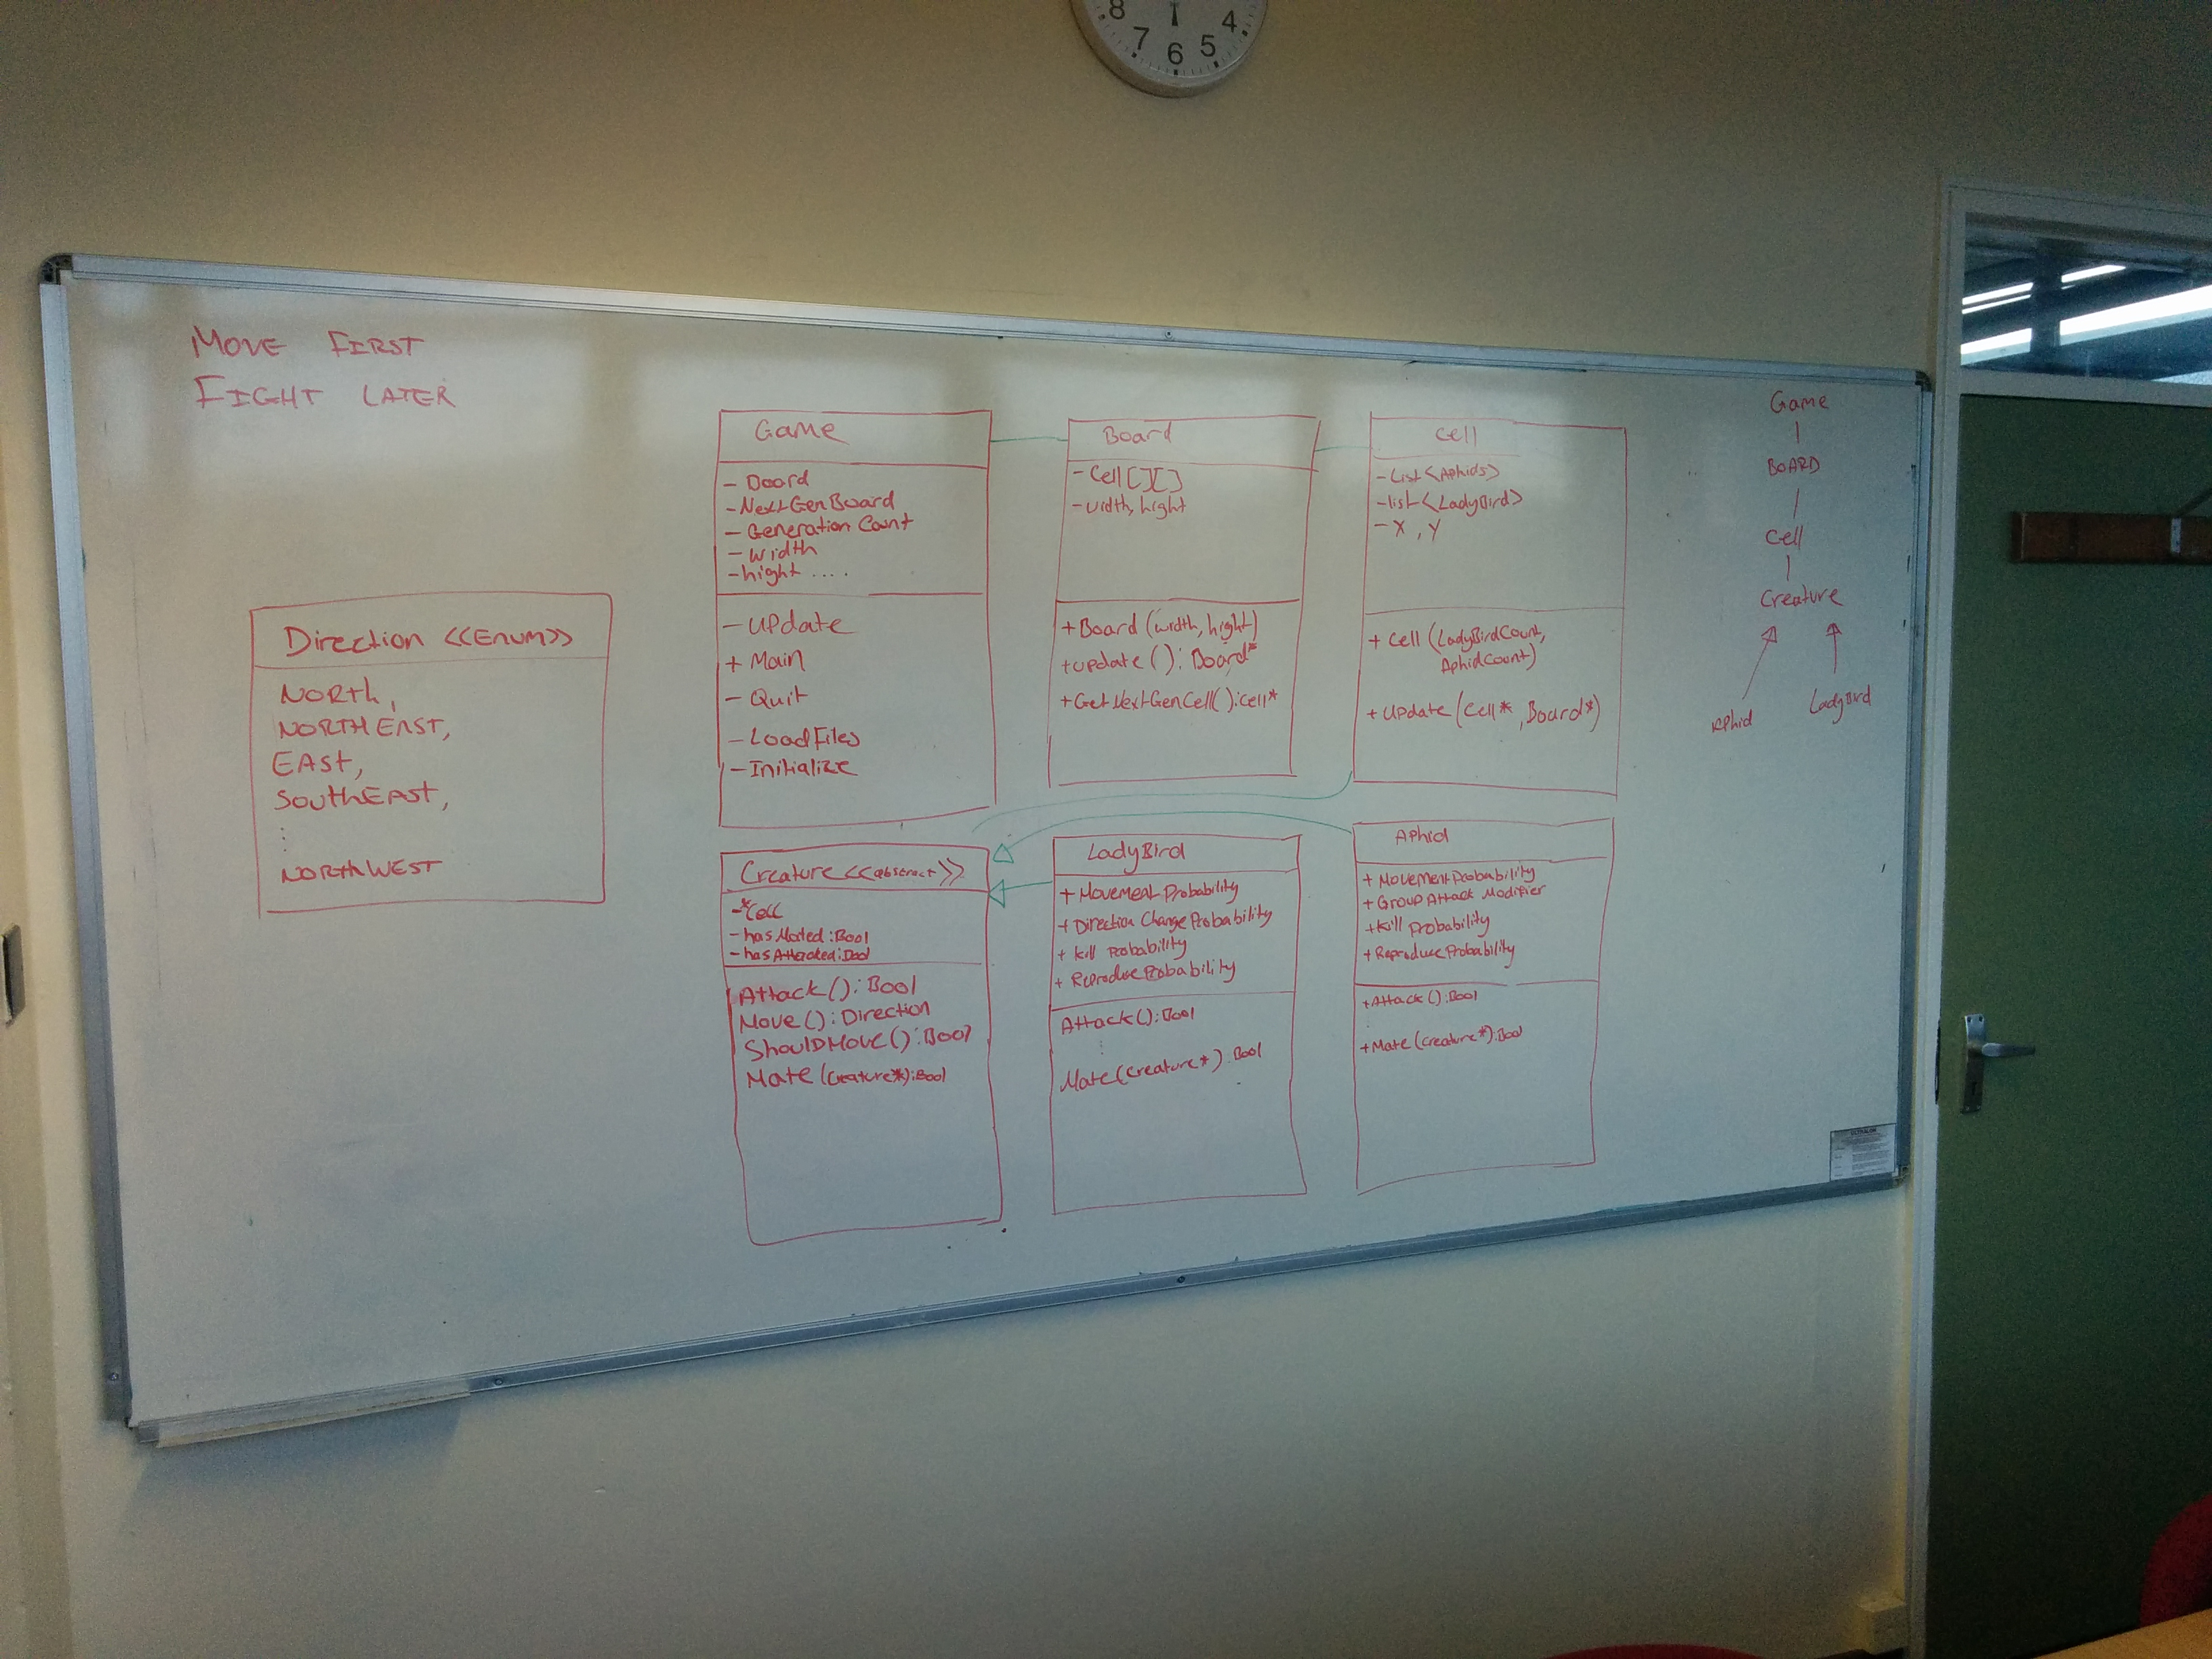
\includegraphics[scale=0.10]{design.jpg}
  \caption{initial design, full res image available in docs folder \label{overflow}}
  \end{figure}
  %\end{landscape}

  In the design I have a Creature class as this is strongly hinted at in the specification. From this the ladybirds and aphids inherit some of its properties. However the way I chose to create the application, using static variables in the aphids and ladybirds class, there isn't really a need for the creature class as the aphids and ladybirds don't really have any shared properties. This makes the project less abstracted and polymorphic which is an issue for maintainability and expansion of features. 

  The Ladybird and Aphid class contain some simple functions that determine where they move to and if they have killed, depending on the static variables defined by the config files.

  \section{Implementation}
Creating the application was a challenge, as I had to implement my solution and learn C++ as I went along! The first stage was to create a board and get it to print out in a nice format. This was mainly so that debugging the project would be easier and the end result would look more appealing. I decided upon using bash colour codes and special characters to format the output. This is because I am working on the linux platform and the specification didn't have any requirement for what platform the application should run on. Using this formatting does make it harder to port the project to Windows, however that is not in the scope of this project.

\end{document}
